\documentclass{article}
\usepackage[paperwidth=28cm,paperheight=10cm,margin=0cm]{geometry}
\usepackage[T1]{fontenc}
\usepackage{lmodern}
\usepackage{xcolor}
\usepackage{tikz}
\usetikzlibrary{arrows.meta,positioning,fit,backgrounds}
\pagestyle{empty}
\definecolor{cbBlue}{HTML}{0173B2}
\definecolor{cbOrange}{HTML}{DE8F05}
\definecolor{cbGreen}{HTML}{029E73}
\definecolor{ink}{HTML}{303840}
\definecolor{muted}{HTML}{5D6872}
\definecolor{trainBg}{HTML}{F4F7FA}
\definecolor{testBg}{HTML}{FAF8F3}
\definecolor{modelBg}{HTML}{E7F1F8}
\definecolor{applyBg}{HTML}{E8F3E8}
\definecolor{perfBg}{HTML}{FFF0D5}
\begin{document}
\noindent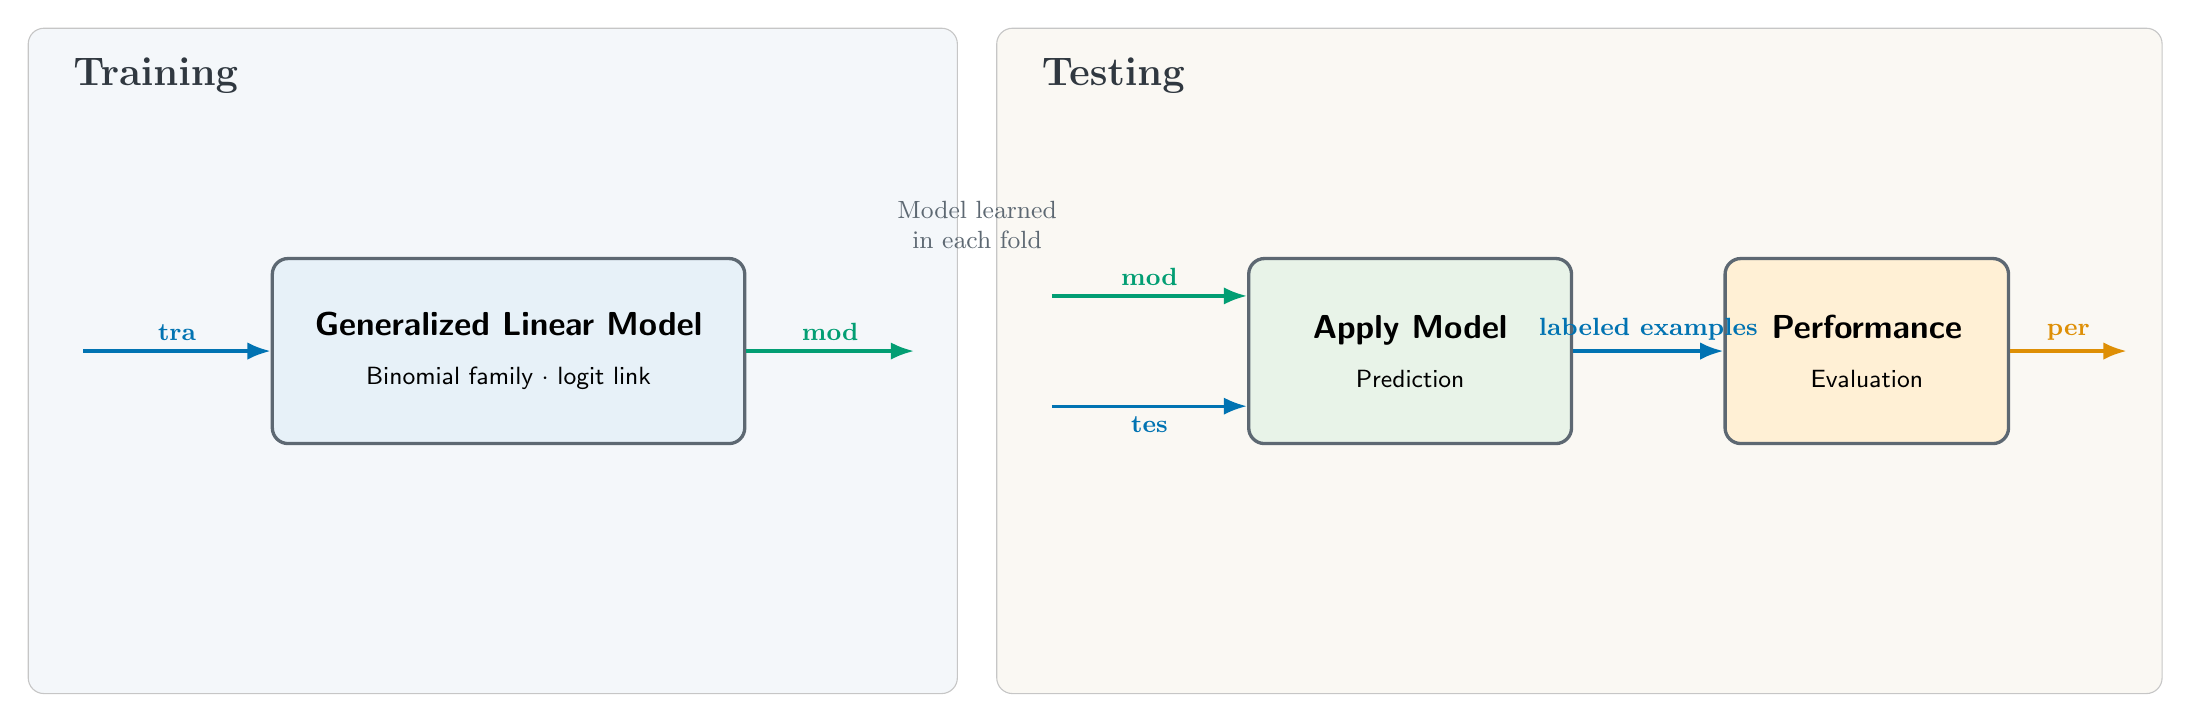
\begin{tikzpicture}[x=1cm,y=1cm,>=Latex,font=\sffamily,
  box/.style={draw=muted,rounded corners=2mm,very thick,minimum height=2.35cm,align=center},
  flow/.style={-Latex,very thick},
  port/.style={font=\bfseries\small}]
  \fill[trainBg,rounded corners=2mm] (0.45,0.7) rectangle (12.25,9.15);
  \draw[gray!45,rounded corners=2mm] (0.45,0.7) rectangle (12.25,9.15);
  \fill[testBg,rounded corners=2mm] (12.75,0.7) rectangle (27.55,9.15);
  \draw[gray!45,rounded corners=2mm] (12.75,0.7) rectangle (27.55,9.15);
  \node[anchor=west,font=\bfseries\Large,text=ink] at (0.9,8.55) {Training};
  \node[anchor=west,font=\bfseries\Large,text=ink] at (13.2,8.55) {Testing};

  \node[box,fill=modelBg,minimum width=6.0cm] (glm) at (6.55,5.05)
    {\bfseries\large Generalized Linear Model\\[2mm]\small Binomial family $\cdot$ logit link};
  \draw[flow,cbBlue] (1.15,5.05) -- node[port,above,text=cbBlue] {tra} (glm.west);
  \draw[flow,cbGreen] (glm.east) -- node[port,above,text=cbGreen] {mod} (11.7,5.05);
  \node[font=\small,text=muted,align=center] at (12.5,6.65) {Model learned\\in each fold};

  \node[box,fill=applyBg,minimum width=4.1cm] (apply) at (18.0,5.05)
    {\bfseries\large Apply Model\\[2mm]\small Prediction};
  \node[box,fill=perfBg,minimum width=3.6cm] (perf) at (23.8,5.05)
    {\bfseries\large Performance\\[2mm]\small Evaluation};
  \draw[flow,cbGreen] (13.45,5.75) -- node[port,above,text=cbGreen] {mod} (apply.west |- 0,5.75);
  \draw[flow,cbBlue] (13.45,4.35) -- node[port,below,text=cbBlue] {tes} (apply.west |- 0,4.35);
  \draw[flow,cbBlue] (apply.east) -- node[port,above,text=cbBlue] {labeled examples} (perf.west);
  \draw[flow,cbOrange] (perf.east) -- node[port,above,text=cbOrange] {per} (27.1,5.05);
\end{tikzpicture}
\end{document}
